\chapter{Properties of Functions}

\section{Maxima and Minima}

Find the coordinates of the any relative maxima or minima. Round to 3 decimal places when necessary.

\begin{enumerate}
\item $f(x) = x^2 - 3x^2 + 5$
\item $g(x) = -0.4x^3 + 0.6x^2 + 3x - 2$
\setcounter{Review}{\value{enumi}}
\end{enumerate}

\begin{enumerate}
\setcounter{enumi}{\value{Review}}
\item The concentration $C$ of a medication in the bloodstream $t$ hours after being administered can be modeled by
\[ C(t) = -0.002t^4 + 0.039t^3 - 0.285t^2 + 0.766t + 0.085, \quad t \geq 0 \]

After how many hours will the concentration be the highest?
\end{enumerate}

\section{Increasing, Decreasing, and Constant Intervals}

Find the intervals in which each is increasing or decreasing. Round to 3 decimal places when necessary.

\begin{enumerate}
\item $f(x) = x^2 - 3x^2 + 5$
\item $g(x) = -0.4x^3 + 0.6x^2 + 3x - 2$
\end{enumerate}

\section{Miscellaneous}

Use the graph of $y = f(x)$ below to answer questions 1--10. Write your answers using interval notation.
\begin{center}
    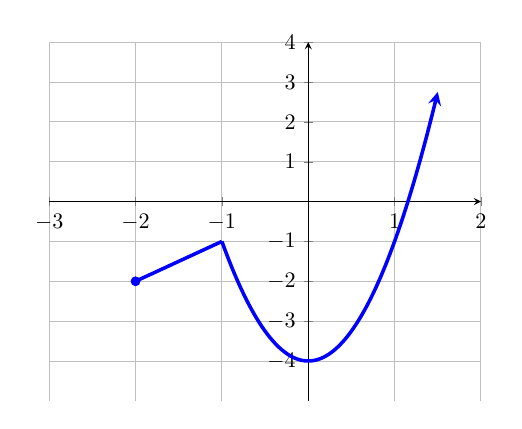
\begin{tikzpicture}[>=stealth, scale=0.8]
    \begin{axis}
    [axis lines = middle, grid,
    xmin = -3, xmax = 2, ymin = -5, ymax = 4,
    % xtick = {-2.5,-2,...,1.5}, 
    ytick = {-4,-3,...,4}
    ]
    \addplot[ultra thick, color=blue,samples=200, domain=-2:-1] {x};
    \addplot[->, ultra thick, color=blue, samples=200, domain=-1:1.5] {3*x^2-4};
    \addplot[color=blue, mark = *] coordinates {(-2,-2)};
    \end{axis}
    \end{tikzpicture}
\end{center}

\begin{enumerate}
\item Domain of $f$
\item Range of $f$
\item Relative Minimum
\item Relative Maximum
\item $f(1)$
\item $f(0)$
\item Increasing Interval(s)
\item Decreasing Interval(s)
\item Absolute Maximum
\item Absolute Minimum
\end{enumerate}

\newpage

\textsc{Properties of Functions Key} 

\section*{Maxima and Minima}

\begin{enumerate}
\item Rel max @ $(0,5)$; No rel min
\item Rel max @ $(2.158, 3.248)$; Rel min @ $(-1.158, -4.048)$
\item About 2.16 hours
\end{enumerate}

\section*{Increasing, Decreasing, and Constant Intervals}

\begin{enumerate}
\item Increasing: $(-\infty, 0)$ \quad Decreasing: $(0, \infty)$
\item Increasing: $(-1.158, 2.158)$ \quad Decreasing: $(-\infty, -1.158) \cup (2.158, \infty)$
\end{enumerate}

\section*{Miscellaneous}

\begin{enumerate}
    \item $[-2, \infty)$
    \item $[-4, \infty)$
    \item $(0, -4)$
    \item $(-1,-1)$
    \item $-1$
    \item $-4)$
    \item $(-2, -1) \cup (0, \infty)$
    \item $(-1,0)$
    \item $(0,-4)$
    \item None
\end{enumerate}